\documentclass{article}
\usepackage[UTF8]{ctex}
\usepackage{amsmath}
\usepackage{amssymb}
\usepackage{graphicx}
\usepackage{float}
\usepackage{datetime}
\usepackage{geometry}

\geometry{a4paper, top=2.54cm, bottom=2.54cm, left=3.18cm, right=3.18cm}

\author{刘思昀 SLST 2022522011}

\title{General Physics II 用霍尔效应测量螺线管磁场}

\begin{document}

\date{\formatdate{3}{4}{2024}}

\maketitle

\section{磁感应强度$B$与霍尔电势差$U_H$的关系,并校正霍尔传感器灵敏度}

调节电压输出为$5.0V$,此时数字电压表上显示OUT-和V-间的电压为$2.502V$

将霍尔传感器置于$X = 15cm$处,改变励磁电流,测量$U- I_M$的关系
\begin{figure*}[htbp]
    \centering
    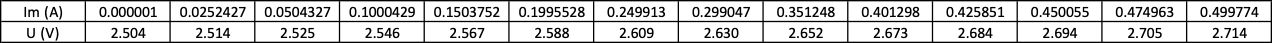
\includegraphics[width=0.99\textwidth]{B-UH.png}
    \caption{磁感应强度$B$与霍尔电势差$U_H$的关系}
\end{figure*}

绘制磁感应强度$B$与霍尔电势差$U_H$的曲线,并进行线性拟合
\begin{figure*}[htbp]
    \centering
    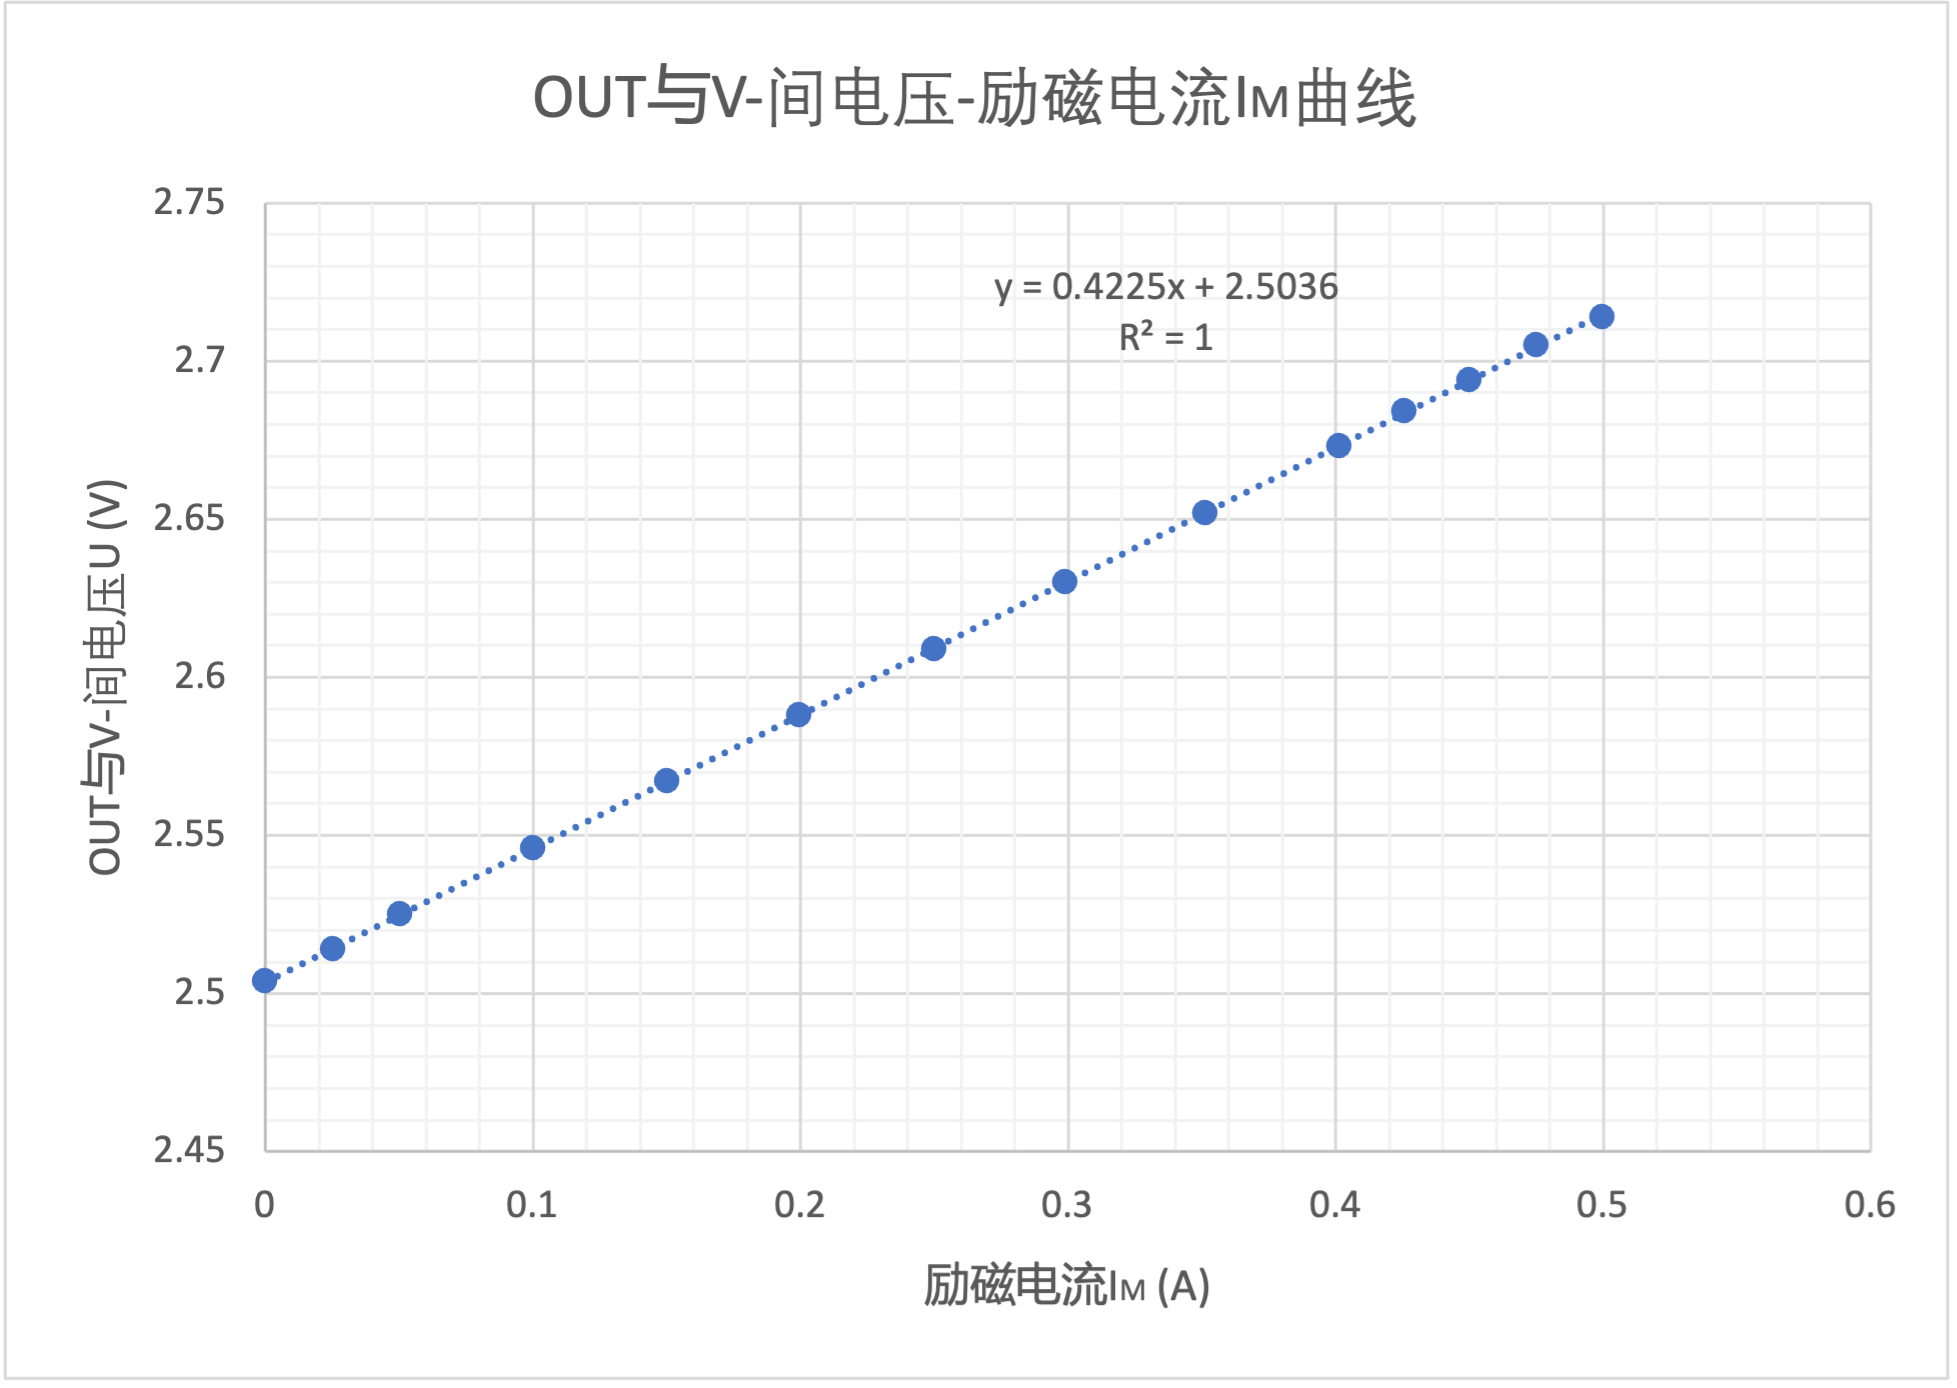
\includegraphics[width=0.95\textwidth]{curve1.png}
    \caption{磁感应强度$B$与霍尔电势差$U_H$的曲线}
\end{figure*}
拟合结果:
\begin{align*}
    y &= 0.422x + 2.504 \\ 
    R^2 &= 1 \\
    Thus, &\frac{\Delta U}{\Delta I_M} = 0.422
\end{align*}

$\mu_0$为真空磁导率,$\mu_0 = 4\pi \times 10^{-7} T \cdot m/A, N=3000, L = 0.260 m, D = 3.50 cm$,由此可以计算螺线管中心磁场强度理论值:
\begin{align*}
    B_{theory} &= \frac{\mu_0 N I_M}{\sqrt{L^2 + \bar{D}^2}} \\
    &= \frac{3000}{\sqrt{0.260^2 + (3.5 \times )^2}} 4\pi \times 10^{-7} I_M \\
    B_{theory} / I_M &= 1.437 \times 10^{-2} \\
    K &= \frac{I_M}{B_{theory}} \cdot \frac{\Delta U}{\Delta I_M} \\
    &= \frac{1}{1.437 \times 10^{-2}} \times 0.422 \\
    &= 29.4 V/T = 2.94 mV/G
\end{align*}

\section{测量通电螺线管内磁感应强度分布}
励磁电流保持不变,为$I_M = 0.249887A$

改变霍尔元件位置:在 $0-7cm, 25-30cm$ 范围内,每隔 $0.2cm$ 记录一个数据;在 $7-9cm, 23-25cm$ 范围内,每隔 $0.4cm$ 记录一个数据;在 $9-23cm$ 范围内,每隔 $1.0cm$ 记录一个数据

利用已经计算出的灵敏度$K = 29.4 V/T$,计算磁感应强度$B$的数值
\begin{align*}
    K &= \frac{\sqrt{L^2 + D^2}}{\mu_0 N} \cdot \frac{\Delta U}{\Delta I_M} \\
    &= \frac{I_M}{B} \cdot \frac{U'}{I_M} \\
    &= \frac{U'}{B} \\
    B &= \frac{U'}{K} = \frac{1000U'}{29.4} mT
\end{align*}

\begin{figure*}[htbp]
    \centering
    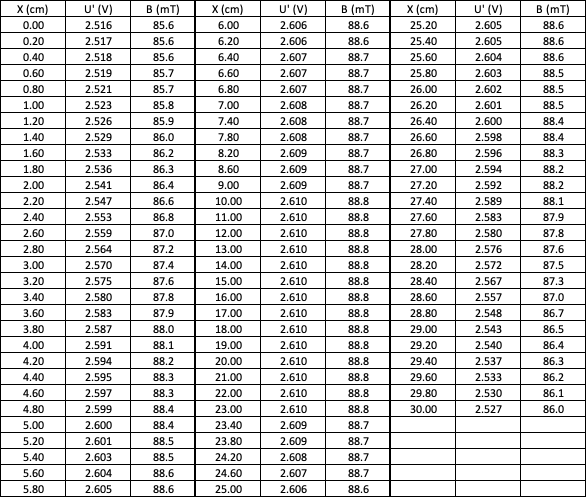
\includegraphics[width=0.9\textwidth]{B_value.png}
    \caption{各点的磁感应强度}
\end{figure*}

根据轴线上各点的磁感应强度,绘制螺线管轴线上磁场的分布曲线

\begin{figure*}[htbp]
    \centering
    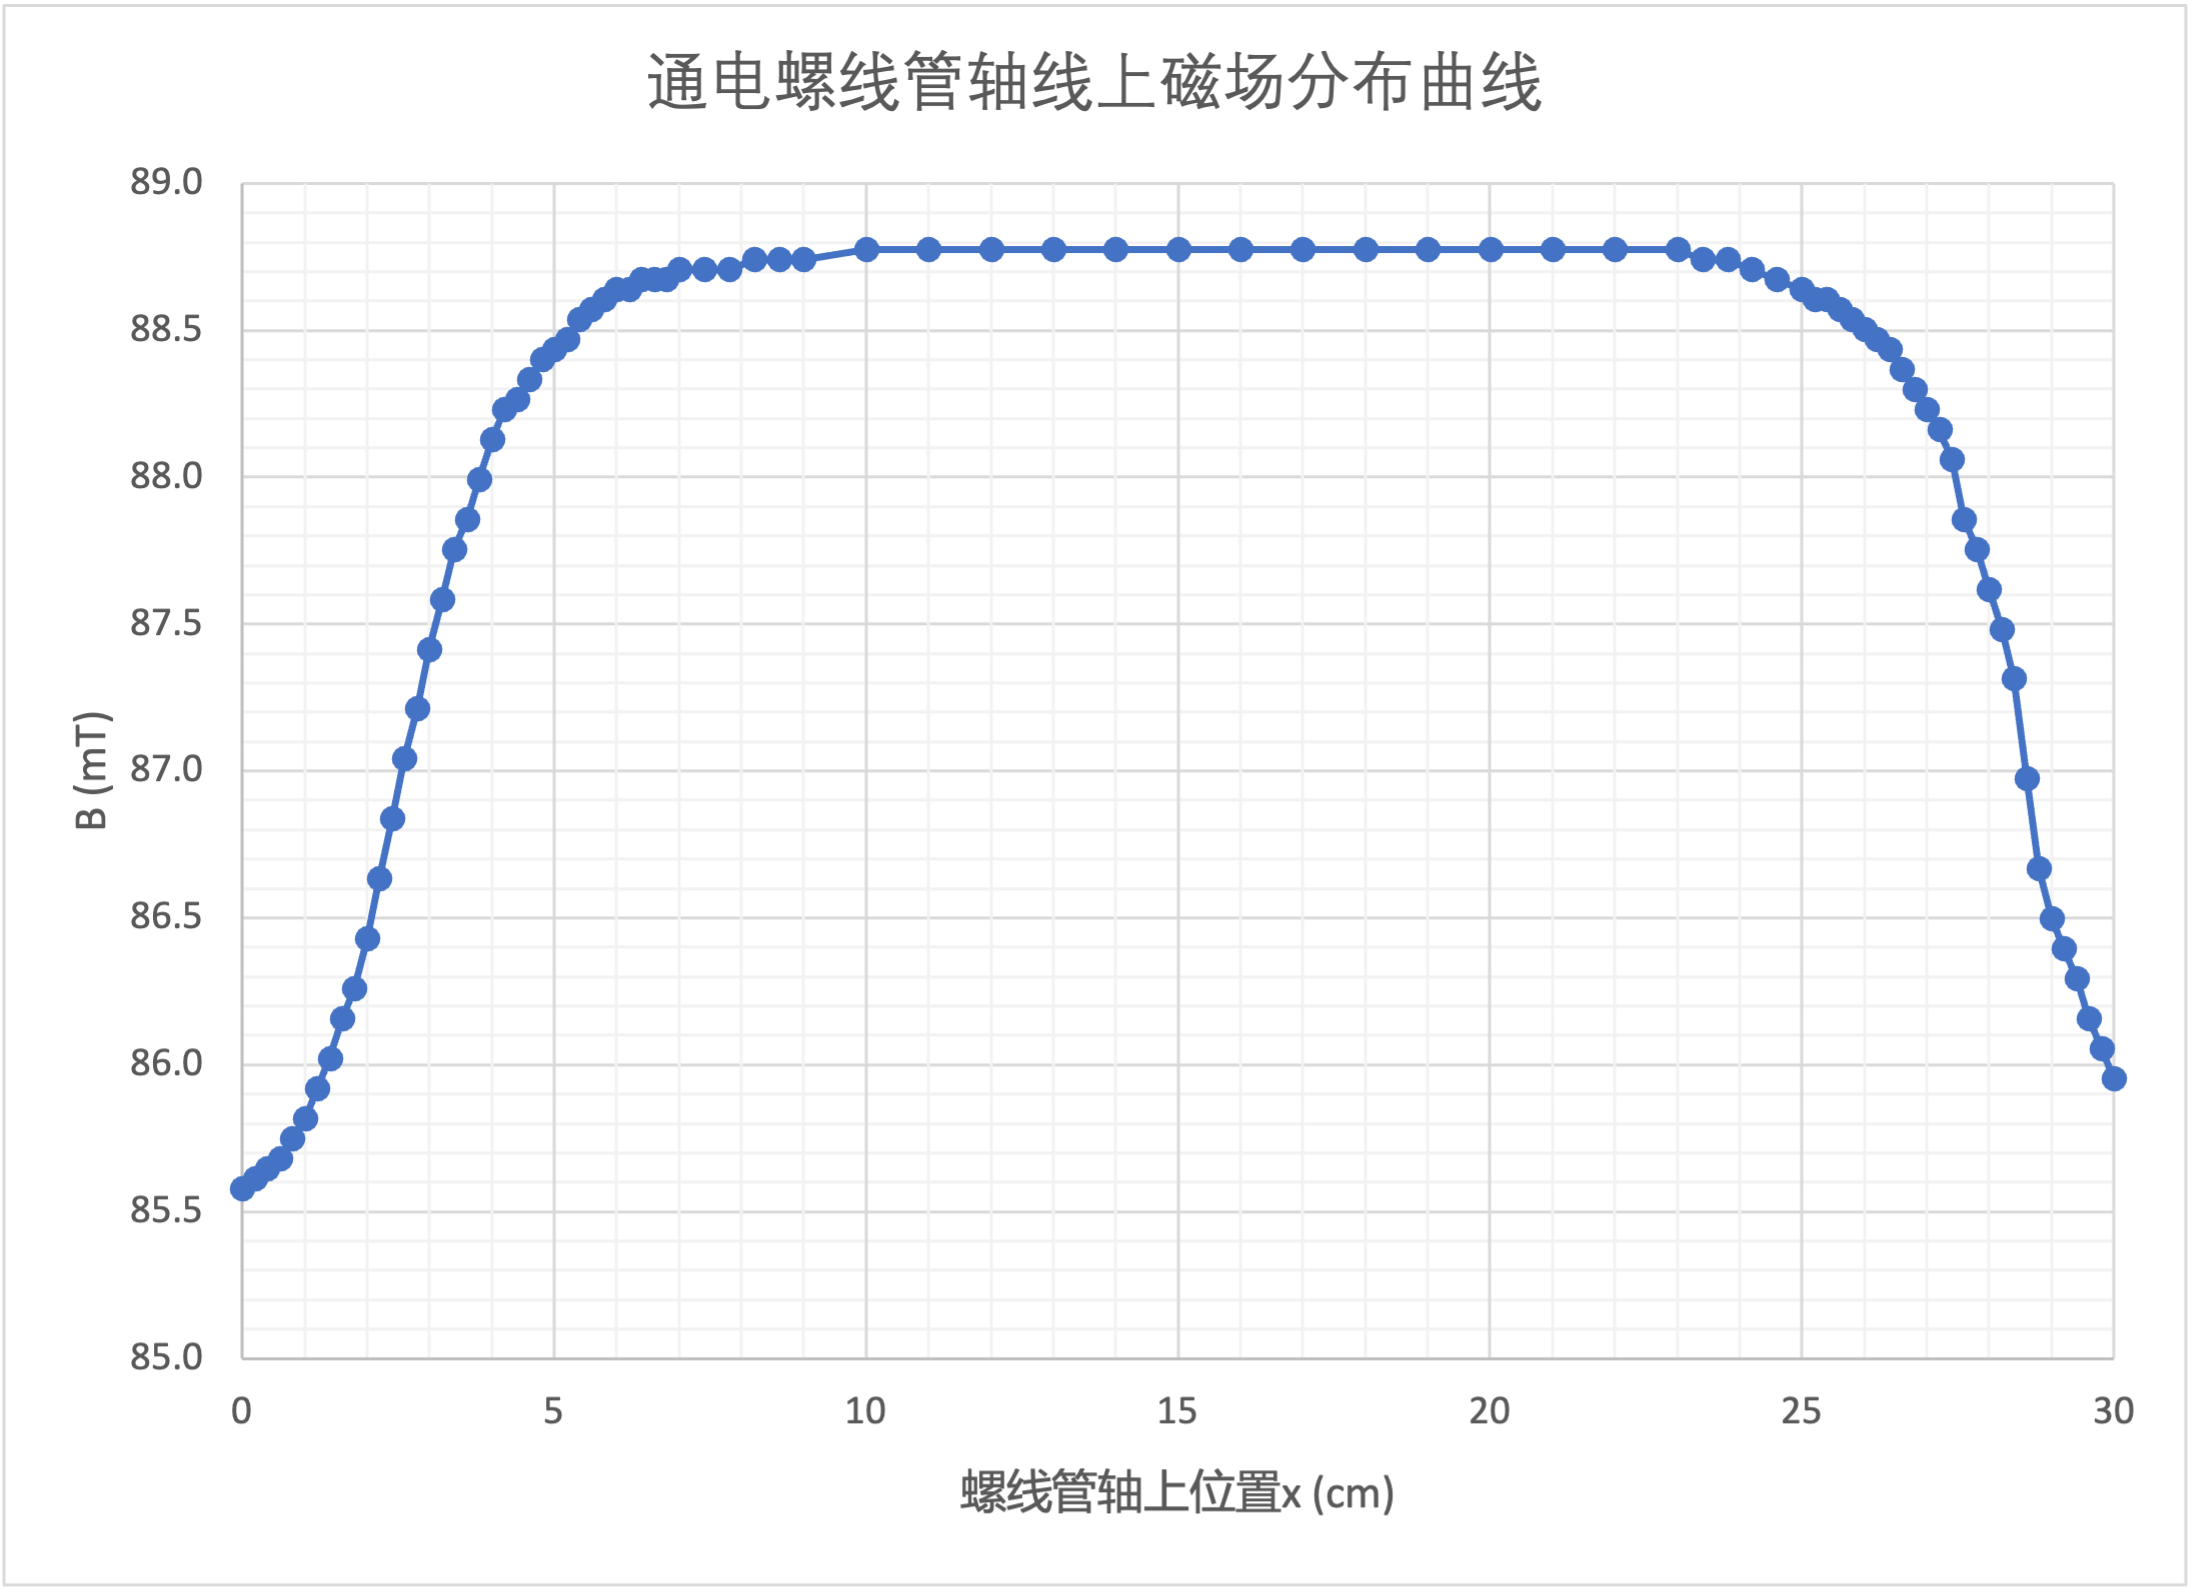
\includegraphics[width=0.9\textwidth]{B_plot.png}
    \caption{通电螺线管轴线上磁场分布曲线}
\end{figure*}

可以观察到,在通电螺线管中间位置,磁感应强度较大且均匀,在两端会有磁感应强度的减小

\newpage

\section{思考题}
\subsection{$I_M=0$ 时,由于地磁场的存在,$U_H$ 不一定为0,怎样消除地磁场的影响?}
可以采用电压补偿法。通过设置一个剩余电压补偿器,可以调整电路以消除或补偿地磁场引起的霍尔电压,使得在没有磁场作用(包括地磁场)的情况下,霍尔传感器的输出电压调整为一个标准值,从而确保测量的准确性。

\subsection{自行设计实验,测量地磁场,计算当地的磁倾角。}
将霍尔传感器安装在三脚架或稳固支架上,并确保它可以绕一个水平轴旋转。霍尔传感器的敏感面应该能够从水平位置旋转到垂直位置。在没有外部磁场的情况下,调整霍尔传感器输出电压至标准值,以校准仪器并消除剩余电压的影响。

将霍尔传感器的敏感面调整至水平方向,测量并记录此时的霍尔电压,通过已知的霍尔传感器灵敏度转换成磁场强度,这可以反映地磁场水平分量的大小。将霍尔传感器的敏感面调整至垂直方向,测量并记录此时的霍尔电压,并转换成磁场强度,这可以反映地磁场垂直分量的大小。

地磁场的总强度:
\begin{equation*}
    B_{total} = \sqrt{B_{vertical}^2 + B_{horizontal}^2}
\end{equation*}

磁偏角:
\begin{equation*}
    \theta = arctan \left( \frac{B_{vertical}}{B_{horizontal}} \right)
\end{equation*}

\subsection{改变磁场方向,讨论对补偿电压有什么影响。}
霍尔效应描述了当一个带电粒子流在一个磁场中流动时,它们会受洛伦兹力的作用。这个力会导致电荷在材料的一侧积累,从而在垂直于电流和磁场的方向上产生电压差,即霍尔电压。补偿电压是用来抵消由于磁场引起的这个电压差的。

霍尔电压$U_H = \frac{B \cdot I \cdot R_H}{d}$从这个公式可以看出,霍尔电压与磁场强度成正比,并且方向也有关。

改变磁场方向的影响:

\begin{itemize}
    \item 霍尔电压的大小取决于磁场分量,该分量垂直于电流方向和材料的厚度方向。如果磁场方向完全平行于电流流动的方向,那么理论上不会产生霍尔电压,因为洛伦兹力为零。
    \item 改变磁场方向会改变洛伦兹力的方向,从而改变电荷在材料中的分布方向,这直接影响到霍尔电压的极性。如果磁场方向逆转,霍尔电压的极性也会逆转。
    \item 为了抵消霍尔电压并使输出电压维持在一个恒定值,补偿电压的大小和方向都需要随着磁场方向的改变而调整。如果磁场方向改变导致了霍尔电压极性的逆转,补偿电压也必须逆转其极性来保持输出电压稳定。
\end{itemize}。

\section{分析与讨论}
\begin{itemize}
    \item 若在通电螺线管中间位置,电压表示数仍有大量波动,可能是霍尔传感器仪器本身存在问题
\end{itemize}

\end{document}